\chapter{Il gestionale}\label{chapter:gestionale}
Il gestionale interno di Dieffetech è stato rifatto per rispondere alle esigenze di efficienza, scalabilità e semplicità di gestione che l'azienda aveva maturato nel corso degli anni.

Questo capitolo descrive le motivazioni dietro il rifacimento del sistema e le tecnologie adottate, concentrandosi sulle principali differenze tra il vecchio e il nuovo gestionale, con un focus su Laravel e React, nonché sugli strumenti utilizzati per il suo sviluppo.

\section{Cause della Ristrutturazione}\label{sec:cap_sec_subsec_perchè}
Il rifacimento del gestionale interno di Dieffetech è stato motivato dalla necessità di modernizzare un sistema che, sebbene funzionante, aveva raggiunto dei limiti a causa delle tecnologie obsolete utilizzate.

In precedenza, il gestionale si basava su Yii per il backend, con l'utilizzo di JavaScript, HTML e CSS per il frontend. Sebbene queste tecnologie fossero adatte per le esigenze iniziali dell'azienda, non garantivano più la scalabilità e le prestazioni necessarie per gestire un flusso di lavoro crescente e un numero sempre maggiore di dati da elaborare.

La decisione di adottare Laravel per il backend e React per il frontend è stata determinata dalla necessità di rendere il sistema più robusto, flessibile e facilmente manutenibile.

Laravel, con la sua architettura solida e il suo ecosistema di strumenti, ha consentito di creare un backend più sicuro ed efficiente. React, d'altra parte, ha permesso di migliorare l'interfaccia utente, rendendola dinamica e reattiva, con tempi di risposta molto più rapidi rispetto alla versione precedente. Questa combinazione di tecnologie ha portato a una gestione centralizzata delle informazioni e a una migliore esperienza utente per i dipendenti di Dieffetech.

\section{Confronto tra il Vecchio e il Nuovo Gestionale}
Il rifacimento del gestionale ha comportato numerosi cambiamenti rispetto alla versione precedente. Le principali differenze riguardano sia la tecnologia utilizzata che l'esperienza dell'utente.

Qui di seguito sono descritte le differenze principali tra il vecchio e il nuovo sistema:
\subsection{Scelte Tecnologiche}
\begin{itemize}
    \item \textbf{Vecchio sistema}: Il precedente sistema si avvaleva del framework \texttt{Yii} per il backend, mentre per il frontend si utilizzavano tecnologie come \texttt{JavaScript}, \texttt{HTML} e \texttt{CSS}.
    Sebbene queste tecnologie fossero adeguate per l'inizio, si rivelavano meno scalabili e modulari man mano che cresceva la complessità del sistema.
    \item \textbf{Nuovo sistema}: Il nuovo gestionale utilizza \texttt{Laravel} per il backend e \texttt{React} per il frontend. \texttt{Laravel} offre un'architettura robusta per la gestione delle operazioni lato server, mentre \texttt{React} consente un'interfaccia utente più dinamica e reattiva, migliorando l'esperienza complessiva dell'utente.
\end{itemize}

\subsection{Interfaccia utente}

\begin{itemize}
    \item \textbf{Vecchio sistema}: L’interfaccia utente risultava funzionale, ma limitata in termini di flessibilità. Le interazioni non erano molto fluide e il sistema non era progettato per adattarsi facilmente alle evoluzioni delle necessità aziendali.
    \item \textbf{Nuovo sistema}: L'interfaccia utente è stata riprogettata per essere più moderna, interattiva e user-friendly. L'adozione di \texttt{React}, ha reso le transizioni tra le pagine significativamente più rapide, migliorando l'esperienza dell'utente finale e riducendo il rischio di errori.
\end{itemize}

\subsection{Prestazioni}

\begin{itemize}
    \item \textbf{Vecchio sistema}: Le prestazioni del vecchio sistema erano sufficienti ma tendenti a rallentare quando il volume di dati e richieste cresceva, soprattutto nelle operazioni di gestione dei dati.
    \item \textbf{Nuovo sistema}: "Il nuovo sistema garantisce un notevole miglioramento delle prestazioni, grazie a un'architettura più efficiente.
    \texttt{React} migliora la velocità di rendering delle pagine, mentre \texttt{Laravel} ottimizza la gestione delle richieste lato server, riducendo i tempi di risposta e aumentando la reattività.
\end{itemize}

\subsection{Sicurezza}

\begin{itemize}
    \item \textbf{Vecchio sistema}: Il sistema precedente non offriva gli stessi livelli di protezione e gestione sicura degli accessi che sono oggi richiesti per proteggere i dati sensibili.
    \item \textbf{Nuovo sistema}: Grazie all’integrazione di \texttt{Laravel Sanctum}, il nuovo gestionale offre un sistema di autenticazione sicuro basato su token CSRF, migliorando la protezione dei dati aziendali e garantendo un livello di sicurezza più elevato.
\end{itemize}

\section{React}\label{sec:cap_sec_subsec_react}
React è una libreria JavaScript sviluppata da Jordan Walke (un software engineer di Meta) nel 2013, progettata per creare interfacce utente (UI) reattive e dinamiche. Si distingue principalmente per la sua capacità di aggiornare in modo efficiente solo le porzioni di UI che cambiano, riducendo così il carico sulle risorse del sistema e migliorando l'esperienza utente. Utilizzando un approccio basato su componenti, React consente agli sviluppatori di suddividere le interfacce in parti modulari, ognuna con il proprio stato e comportamento, che possono essere riutilizzate e testate in modo indipendente.

Una delle caratteristiche distintive di React è il Virtual DOM (Document Object Model), un'astrazione che permette di migliorare le performance durante il rendering delle interfacce utente. Invece di aggiornare direttamente il DOM del browser, React prima aggiorna una rappresentazione in memoria (il Virtual DOM) e poi calcola la differenza con il DOM effettivo, applicando solo le modifiche necessarie. Questo approccio riduce significativamente i tempi di rendering, soprattutto per le applicazioni con una grande quantità di dati e componenti dinamici.

React segue il paradigma della programmazione dichiarativa, in cui gli sviluppatori descrivono come dovrebbe apparire la UI in ogni stato e React si occupa di aggiornare il DOM in modo efficiente quando lo stato cambia. Questo paradigma rende il codice più leggibile, facilmente manutenibile e scalabile, particolarmente utile in progetti di grandi dimensioni.

L'adozione di React nel rifacimento del gestionale di Dieffetech ha portato a una notevole miglioria nell'interazione dell'utente con il sistema. Grazie alla sua velocità di rendering e alla modularità dei componenti, l'interfaccia utente è diventata più fluida e reattiva, con una gestione dinamica dei dati in tempo reale. React ha permesso di creare un'esperienza più coinvolgente per gli utenti, riducendo al minimo i tempi di attesa e migliorando l'usabilità complessiva della piattaforma.

\subsection{Architettura di un Progetto}
Un tipico progetto React ha la seguente struttura delle cartelle:

\begin{verbatim}
    react/
    |-- node_modules/
    |-- public/
    |   |-- index.html
    |   `-- favicon.ico
    |-- src/
    |   |-- components/
    |   |-- forms/
    |   |-- tables/
    |   |-- styles/
    |-- .gitignore
    |-- .env
    |-- package-lock.json
    |-- package.json
    `-- README.md
    \end{verbatim}
La cartella \texttt{src} è il cuore del progetto React, poiché contiene tutti i file sorgente necessari per il funzionamento dell'applicazione. Al suo interno, la cartella \texttt{components/} raccoglie tutti i componenti riutilizzabili, come il \texttt{CrudDataTable}, che gestisce le tabelle dinamiche per la visualizzazione e l'interazione con i dati.
Inoltre, all'interno della cartella \texttt{src/}, esistono altre due cartelle fondamentali:

\begin{itemize}
    \item \textbf{\texttt{forms/}}: Contiene tutti i moduli (form) necessari per la creazione e gestione di nuovi dati. Ogni tabella avrà il proprio form dedicato, consentendo una gestione centralizzata e modulare della creazione dei record.
    \item \textbf{\texttt{tables/}}: Contiene i componenti che gestiscono la visualizzazione delle tabelle. Questi componenti sono responsabili della gestione dei dati provenienti dal backend, e vengono visualizzati all'interno delle diverse tab nel \texttt{baseMenu} del gestionale, permettendo una navigazione fluida tra le varie sezioni.
\end{itemize}

Questa organizzazione modulare permette una gestione chiara e scalabile del codice, semplificando l'aggiornamento e la manutenzione dell'applicazione.

\section{Laravel}\label{sec:laravel_laravel}
Laravel è un framework PHP open-source progettato per semplificare lo sviluppo di applicazioni web. Creato da Taylor Otwell nel 2011, Laravel ha guadagnato rapidamente popolarità grazie alla sua sintassi elegante, alla ricca documentazione e alla robusta architettura. È stato pensato per facilitare la gestione di operazioni comuni come la gestione delle rotte, l'autenticazione degli utenti, il trattamento delle richieste HTTP e la gestione dei database, riducendo la complessità del codice.

Una delle caratteristiche distintive di Laravel è il suo \textit{Eloquent ORM} (Object-Relational Mapping), che permette una gestione semplice e intuitiva dei dati in un database relazionale. Inoltre, Laravel include funzionalità avanzate come la gestione delle code di lavoro, il supporto per le migrazioni di database e il sistema di notifiche.

Laravel è strutturato per essere altamente modulare, consentendo agli sviluppatori di costruire applicazioni scalabili e mantenibili con facilità. La sua architettura basata su MVC (Model-View-Controller) aiuta a separare la logica di presentazione dalla logica applicativa, migliorando la leggibilità e la manutenzione del codice.
\begin{figure}[H]
	\centering
	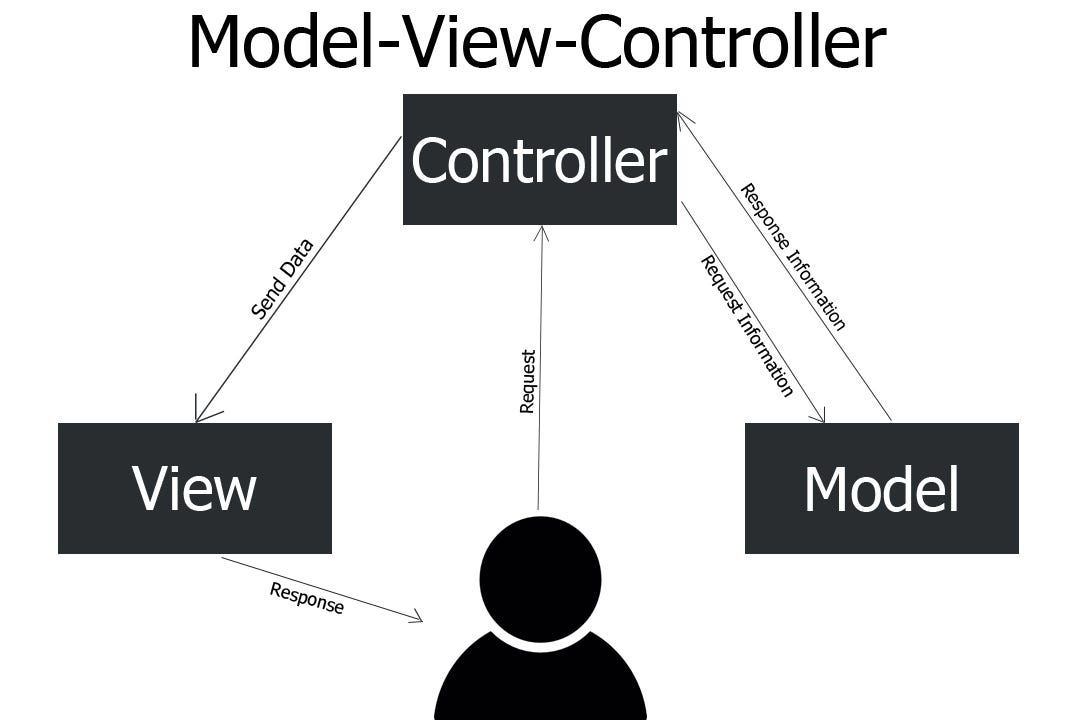
\includegraphics[width=0.7\textwidth]{immagini/MVC.jpg}
	\label{fig:mvc_pattern}
\end{figure}
In questa sezione, vedremo i principali vantaggi e componenti che sono inclusi nell'utilizzo di Laravel.
\subsection{Sail}\label{subsec:cap_sec_subsec_sail}
Laravel Sail è un ambiente di sviluppo basato su Docker che semplifica l'installazione e la gestione di un'applicazione Laravel in un container isolato. Con Sail, non è necessario configurare manualmente un ambiente di sviluppo locale, poiché tutto il necessario è già preconfigurato. Questo approccio riduce notevolmente la complessità dell'installazione di servizi come il database, Redis e la coda di lavoro, rendendo più semplice e veloce l'avvio di un nuovo progetto.

Nel contesto del rifacimento del gestionale interno, Sail si è rivelato uno strumento prezioso. Grazie alla sua integrazione con Docker, è stato possibile creare un ambiente di sviluppo replicabile e facilmente configurabile per tutti i membri del team. Ogni sviluppatore, infatti, può eseguire l'applicazione Laravel con un semplice comando, garantendo che l'ambiente di sviluppo sia omogeneo, riducendo il rischio di errori derivanti da differenze nelle configurazioni locali.

Utilizzando Sail, è stato possibile gestire in modo semplice i vari servizi necessari al funzionamento del gestionale, come il database MySQL, Redis per la gestione delle sessioni e altri servizi cruciali per il sistema.
\subsection{Sanctum}\label{subsec:cap_sec_subsec_sanctum}
Laravel Sanctum è una libreria che fornisce un sistema di autenticazione semplice e sicuro per le applicazioni Laravel, pensato per gestire sia l’autenticazione di sessione che l’autenticazione tramite API. Una delle caratteristiche principali di Sanctum è la sua capacità di generare e gestire token di autenticazione per gli utenti che desiderano accedere a determinate risorse protette all’interno dell’applicazione. A differenza di altre soluzioni, Sanctum sfrutta un sistema di token basati su CSRF (Cross-Site Request Forgery), che aiuta a proteggere le applicazioni da attacchi di tipo CSRF, garantendo che le richieste provenienti da client non autorizzati vengano bloccate.

Nel caso del gestionale interno di Dieffetech, Sanctum è stato utilizzato per implementare un sistema di login sicuro. Gli utenti, una volta autenticati tramite la piattaforma, ricevono un token che permette di accedere a specifiche risorse senza dover reinserire le credenziali. Questo sistema di token CSRF protegge ogni richiesta, assicurando che solo gli utenti con un token valido possano interagire con le API e accedere a risorse sensibili.

L’utilizzo di token CSRF è stato fondamentale per garantire una gestione sicura degli accessi, permettendo a ciascun dipendente di operare in modo sicuro e isolato all’interno dell’applicazione. Inoltre, Sanctum si integra facilmente con altre funzionalità di Laravel, come il middleware, per garantire che solo gli utenti autenticati possano accedere a determinate aree del gestionale, senza rischio di esposizione a vulnerabilità CSRF.
\subsection{Telescope}\label{subsec:cap_sec_subsec_telescope}
Laravel Telescope è uno strumento di debugging e monitoraggio che consente di tracciare in tempo reale tutte le richieste HTTP, i log, gli errori, le eccezioni, i job della coda e altro ancora. È un'applicazione dedicata che offre un'interfaccia utente ricca di funzionalità per monitorare e diagnosticare le performance e il comportamento di un'applicazione Laravel durante il processo di sviluppo.

Nel contesto del rifacimento del gestionale, Telescope ha giocato un ruolo cruciale nel monitoraggio delle attività. La capacità di Telescope di tracciare ogni richiesta applicativa ha permesso di analizzare in tempo reale i dettagli operativi, individuando facilmente eventuali anomalie e ottimizzando il sistema. Telescope ha agevolato la risoluzione dei problemi di performance, consentendo una chiara visualizzazione delle query al database, incluse quelle duplicate, facilitando l'individuazione di aree ottimizzabili. La visibilità sulle risorse utilizzate e sulle lentezze nelle operazioni ha permesso di intervenire tempestivamente per ottimizzare il gestionale.

Grazie a questa potente funzionalità di monitoraggio, è stato possibile migliorare significativamente le performance del gestionale, garantendo un'esperienza utente più fluida e reattiva, e ottimizzando il sistema nel suo complesso.
\section{Generazione del CRUD}\label{sec:cap_sec_subsec_crud}
Un CRUD è un acronimo che sta per Create, Read, Update, Delete, che rappresenta le quattro operazioni fondamentali per la gestione dei dati in un'applicazione. Queste operazioni consentono la gestione completa dei dati all'interno di un'applicazione:
\begin{itemize}
    \item \textbf{Create}: Creazione di un nuovo record in un database.
    \item \textbf{Read}: Lettura dei dati da un database.
    \item \textbf{Update}: Modifica o aggiornamento di un record nel database.
    \item \textbf{Delete}: Eliminazione di un record da un database.
\end{itemize}
Prima di iniziare la creazione del CRUD, è essenziale conoscere le convenzioni di nomenclatura (come camelCase o snake\_case, singolare o plurale) poiché i comandi e le funzioni standard di Laravel funzionano correttamente solo se si rispettano tali convenzioni.

Nel contesto del gestionale interno, i CRUD possono essere distinti in due livelli:
\begin{itemize}
    \item \textbf{Primo livello}: Si riferisce ai modelli che vivono di vita propria, come un \textit{progetto}. Questi modelli sono indipendenti e possono esistere senza dipendere da altri modelli.
    \item \textbf{Secondo livello}: Si riferisce ai modelli che esistono solo come figli di altri modelli, come le \textit{task} di un progetto. Le task, infatti, esistono solo se esiste un progetto a cui sono associate.
\end{itemize}
Laravel offre una serie di comandi Artisan che permettono di generare automaticamente i file necessari per la creazione di un CRUD. Questi comandi generano i seguenti file:
\begin{itemize}
    \item \textbf{Model}: Il modello rappresenta la struttura dei dati e va modificato aggiungendo i campi \texttt{fillable}, \texttt{sortable}, \texttt{filterable}, \texttt{searchable}, le relazioni e, se necessario, \texttt{fillableMedia}.
    \item \textbf{Migration}: La migration serve per definire la struttura della tabella del database e aggiungere i campi necessari.
    \item \textbf{Controller}: Il controller implementa le logiche per la creazione, modifica, lettura ed eliminazione dei dati.
    \item \textbf{Policy}: La policy di default viene generata con un \texttt{return true} per ogni azione standard, ma andrà modificata per definire i relativi permessi.
    \item \textbf{Resource}: Un file necessario per far funzionare Laravel correttamente, che non deve essere modificato.
    \item \textbf{Form Request}: Un file vuoto che va completato con tutti i campi che richiedono validazione.
\end{itemize}

Generalmente, in Laravel, esistono comandi specifici come \texttt{php artisan make:controller NomeController}, \texttt{php artisan make:model NomeModello}, ecc., che vengono utilizzati per creare i vari componenti di un'applicazione. Tuttavia, grazie alla creazione di comandi personalizzati, è possibile automatizzare l'intero processo di generazione del CRUD, velocizzando significativamente lo sviluppo del progetto. 

Di seguito sono elencati i comandi di generazione che abbiamo creato, utilizzati per creare in modo rapido i file necessari.
\pagebreak

Per il backend:
\begin{itemize}
    \item \textbf{Primo livello}:
    \begin{itemize}
        \item \texttt{sail artisan app:crud \{name\}}
        \item Esempio: \texttt{sail artisan app:crud Project}
    \end{itemize}
    \item \textbf{Secondo livello}:
    \begin{itemize}
        \item \texttt{sail artisan app:crud \{name\} --parent=\{name\}}
        \item Esempio: \texttt{sail artisan app:crud Task --parent=Project}
    \end{itemize}
\end{itemize}
Per il frontend:
\begin{itemize}
    \item \textbf{Primo livello}:
    \begin{itemize}
        \item \texttt{sail artisan app:crud-fe \{name\}}
        \item Questo comando genera tre file principali:
        \begin{itemize}
            \item \texttt{Pagina}: Una pagina che include il componente della tabella.
            \item \texttt{Tabella}: Un componente \texttt{CrudDataTable} già completo delle props \texttt{title}, \texttt{form} e \texttt{url}. A questo componente vanno aggiunte le colonne necessarie.
            \item \texttt{Form}: Un file che conterrà solo il form, con i vari campi da aggiungere.
        \end{itemize}
        \item Per rendere la nuova sezione raggiungibile, è necessario aggiungere l'apposita voce nel menu di \texttt{apps/react/src/menu/baseMenu.tsx}.
    \end{itemize}
    \item \textbf{Secondo livello}:
    \begin{itemize}
        \item I CRUD nested sono utili quando si lavora con entità annidate. Per esempio, quando all'interno di un progetto esiste una tab \textit{task} che contiene tutte le task associate al progetto.
        \item Comando: \texttt{sail artisan app:crud-fe \{name\} --parent=\{parent\}}
        \item Esempio: \texttt{sail artisan app:crud-fe Task --parent=Project}
    \end{itemize}
\end{itemize}
Questi comandi generano i componenti React per lavorare con le route annidate di Laravel, come nel caso in cui una task dipenda da un progetto. Questo comando predispone già il form e la \texttt{CrudDataTable} per lavorare con la struttura gerarchica delle route.

È fondamentale seguire la convenzione delle route e dei nomi delle risorse durante la creazione dei componenti, affinché la comunicazione tra frontend e backend funzioni correttamente.
\section{API}\label{sec:laravel_api}

Le API (Application Programming Interfaces) sono un insieme di definizioni e protocolli che permettono a diverse applicazioni software di interagire tra loro. Le API definiscono le modalità attraverso cui le informazioni vengono inviate e ricevute tra un client (ad esempio, un'applicazione front-end) e un server (che ospita la logica applicativa e i dati). Le API possono essere utilizzate per esporre funzionalità di un'applicazione in modo che possano essere utilizzate da altre applicazioni.

Nel contesto delle applicazioni web moderne, le API REST (Representational State Transfer) sono tra le più comuni. Le API REST operano attraverso le rotte HTTP standard (GET, POST, PUT, DELETE) per eseguire operazioni CRUD (Create, Read, Update, Delete) sui dati. Ogni rotta API è associata a un'azione, come l'aggiunta di un nuovo record o la lettura di uno esistente.

\subsection{Le rotte API nel progetto}

Le rotte API sono definite nel file di routing del progetto \texttt{routes/api.php}. Ogni rotta è associata a un controller specifico, incaricato della gestione della logica di business per la risorsa corrispondente. All'interno del progetto, sono presenti numerose rotte, ciascuna dedicata a uno o più modelli. Il codice \ref{API} mostra le principali rotte API implementate nel corso dello sviluppo.
\begin{lstlisting}[language=JavaScript, numbers=none, label=API, caption=API]
// Referenti
Route::api('referents', ReferentController::class);
// Appuntamenti
Route::api('appointments', AppointmentController::class);
// Offerte
Route::api('offers', OfferController::class);
// Task
Route::api('tasks', TaskController::class);
// Clienti
Route::api('customers', CustomerController::class);
Route::api('customers.referents', ReferentController::class);
Route::api('customers.appointments', AppointmentController::class);
Route::api('customers.offers', OfferController::class);
Route::api('customers.tasks', TaskController::class);
\end{lstlisting}
\pagebreak
Solitamente, le rotte in Laravel vengono dichiarate con metodi come\\
\texttt{Route::get}, \texttt{Route::post}, e così via. Tuttavia, nel nostro progetto abbiamo creato una rotta personalizzata \texttt{Route::api}, che consente di generare automaticamente tutte le rotte necessarie (come \texttt{index}, \texttt{store}, \texttt{show}, \texttt{update}, \texttt{destroy}) per ogni risorsa con una singola dichiarazione.

\subsection{Funzionamento delle rotte}

Le rotte dichiarate nel file \texttt{routes/api.php} definiscono i punti di accesso per il client per interagire con diverse risorse del sistema:

\begin{itemize}
    \item \texttt{Route::api('referents', ReferentController::class);} definisce una rotta per gestire le operazioni sui referenti. La rotta sarà gestita dal \texttt{ReferentController}.
    \item \texttt{Route::api('appointments', AppointmentController::class);} definisce una rotta che consente di interagire con gli appuntamenti attraverso il \texttt{AppointmentController}.
    \item \texttt{Route::api('offers', OfferController::class);} permette la gestione delle offerte tramite il \texttt{OfferController}.
    \item \texttt{Route::api('tasks', TaskController::class);} definisce una rotta per la gestione dei task, utilizzando il \texttt{TaskController}.
    \item \texttt{Route::api('customers', CustomerController::class);} è la rotta principale per interagire con i clienti, gestita dal \texttt{CustomerController}.
    \item Le rotte con il prefisso \texttt{customers} (come \texttt{customers.referents},\\
    \texttt{customers.appointments}, \texttt{customers.offers}, \texttt{customers.tasks}) definiscono le relazioni tra i clienti e le rispettive risorse. Ad esempio, \texttt{customers.referents} permette di ottenere o gestire i referenti associati a un cliente, \texttt{customers.appointments} gestisce gli appuntamenti di un cliente, e così via.
\end{itemize}

Queste rotte sono associate ai rispettivi controller e sono utilizzate per eseguire operazioni come il recupero, la creazione, l'aggiornamento o la cancellazione dei dati tramite richieste HTTP. Ogni controller gestisce una specifica risorsa e si occupa di applicare la logica di business necessaria per rispondere alle richieste del client.

Inoltre, tutte le rotte API sono avvolte dal middleware \texttt{throttle:api}, che limita il numero di richieste al minuto per evitare attacchi di brute forcing, proteggendo il sistema da un sovraccarico di richieste non autorizzate.\\

Insieme al \texttt{throttle:api}, viene utilizzato anche il middleware \texttt{auth:sanctum}, di cui è stata precedentemente trattata la funzione, per garantire che solo utenti autenticati possano interagire con le API, assicurando così che ogni richiesta provenga da un utente validamente autenticato.
\begin{lstlisting}[language=JavaScript, numbers=none]
Route::middleware('throttle::api', 'auth::sanctum')->group(function() {
  Route::api('route', RouteController::class)
  ...
  ...
})
\end{lstlisting}